\chapter{Flex Coupling Design}

In coupling design, SKF Flex Couplings is used. The catalog provided on \url{https://www.skfptp.com/Publications/Publications#} introduces procedure to select a suitable product. Thus, coupling selection shall follow the instruction on p.60 \cite{skf_2018}

\paragraph{Service factor} The purpose of the mixing tank is not given in design project. Therefore, assuming it is used as a muller mixer, the service factor is 1.5, Table 10, p.88 \cite{skf_2018}.

\paragraph{Design power}
The motor power is $ P_{mo} = 7.14 \unit{kW} $, Table \ref{tab:my-table}.

\paragraph{Coupling size}
The motor speed is $ n_{mo} = 1455 \unit{rpm} $, Table \ref{tab:my-table}. Consulting Table 1, p.61 \cite{skf_2018}, the nearest specification is speed $ n = 1440 \unit{rpm} $ and power rating $ P = 9.95 \unit{kW} $. This results in the coupling size of 50. Also from the table, the nominal torque and max torque are also satisfactory ($ T_{sh} = 46892.66 \unit{N\cdot mm} < 66 \unit{N\cdot m}$).

\paragraph{Bore size}
Hub mounted coupling is used since the shaft is not tapered. Thus, SKF Flex flanges type B size 50 (PHE F50RSBFLG) is selected, p.65 \cite{skf_2018}. From the table on the page, the maximum bore diameter is $ 38\unit{mm} $, which is equal to the motor shaft diameter.

In summary, the flex coupling dimensions and basic physical quantities are specified in the catalog \cite{skf_2018} and product detail report \cite{bibid}.

\begin{figure}[ht]
	\centering
	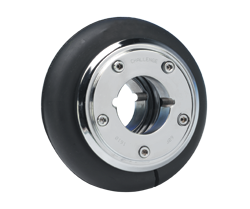
\includegraphics[width=0.5\linewidth]{coupling}
	\caption{Rendered photo of flex coupling PHE F50RSBFLG}
	\label{coupling}
\end{figure}